\documentclass[crop, tikz]{standalone}
\usepackage{tikz}

\usetikzlibrary{positioning}

\begin{document}
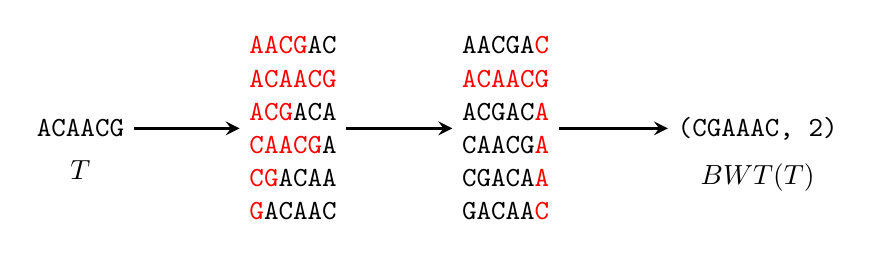
\begin{tikzpicture}[font=\tt]
	\node (T) at (0, 0) {ACAACG};
	\node[below=0.5mm of T] (c1) {$T$};
	\node[align=center] (tbl1) at (2.7, 0) {\textcolor{red}{AACG}AC\\\textcolor{red}{ACAACG}\\\textcolor{red}{ACG}ACA\\\textcolor{red}{CAACG}A\\\textcolor{red}{CG}ACAA\\\textcolor{red}{G}ACAAC};
	\node[align=center] (tbl2) at (5.4, 0) {AACGA\textcolor{red}{C}\\\textcolor{red}{ACAACG}\\ACGAC\textcolor{red}{A}\\CAACG\textcolor{red}{A}\\CGACA\textcolor{red}{A}\\GACAA\textcolor{red}{C}};
	\node[align=left] (BWT) at (8.6, 0) {(CGAAAC, 2)};
	\node[below=0.5mm of BWT] (c2) {$BWT(T)$};
		
	\draw[-stealth, very thick] (T) -- (tbl1);
	\draw[-stealth, very thick] (tbl1) -- (tbl2);
	\draw[-stealth, very thick] (tbl2) -- (BWT);
\end{tikzpicture}
\end{document}
